\documentclass[a4paper,oneside,12pt]{book}

%----------------------------------------------------------------------------------------
%	README!
%   Welcome. It's worth having a read through this file
%   to set up the broad parameters, such as the name of
%   the degree, the school/department, the type of work
%   (dissertation/Final Year Project/report, etc. as well
%   as your own details.
%----------------------------------------------------------------------------------------

%----------------------------------------------------------------------------------------
%	COVER PAGE
%   The cover page is laid out in title/title.tex. You can choose a colour
%   or black and white logo
%----------------------------------------------------------------------------------------

%----------------------------------------------------------------------------------------
%	THESIS INFORMATION
%   Put title, author name, degree, type of work, school, department in here
%   It will be used for the title page and for the embedded PDF information
%----------------------------------------------------------------------------------------

\newcommand{\thesistitle}{Toward a Futuristic Emerald Isle} % Your thesis title, this is used in the title and abstract
\newcommand{\degree}{Computer Engineering} % Your degree name, this is used in the title page and abstract
\newcommand{\typeofthesis}{CG Project} % dissertation, Final Year Project, report, etc.
\newcommand{\authorname}{Chris Casey} % Your name, this is used in the title page and PDF stuff
%% Do not put your Student ID in the document, as TCD will not publish
%% documents that contain both your name and your Student ID.

\newcommand{\keywords}{this, that, more} % Keywords for your thesis
\newcommand{\school}{\href{https://www.tcd.ie/scss/}{School of Computer Science and Statistics}} % Your school's name and URL, this is used in the title page

%% Comment out the next line if you don't want a department to appear
\newcommand{\supervisor}{\href{http://www.scss.tcd.ie/}{Binh-Son Hua}} % Your research group's name and URL, this is used in the title page

\AtBeginDocument{
\hypersetup{pdftitle=\chriscasey20334271} % Set the PDF's title to your title
\hypersetup{pdfauthor=\ChrisCasey} % Set the PDF's author to your name
\hypersetup{pdfkeywords=\keywords} % Set the PDF's keywords to your keywords
\hypersetup{pdfsubject=\CompEngineering} % Set the PDF's keywords to your keywords
}

%% Language and font encodings
\usepackage[T1]{fontenc} 
\usepackage[utf8]{inputenc}
\usepackage[english]{babel}
\usepackage{lipsum}
\usepackage{ragged2e} %allows for text alignment preferences

%% Bibliographical stuff
\usepackage[round,sort,comma,numbers]{natbib}

%% Document size
% include showframe as an option if you want to see the boxes
\usepackage[a4paper,top=2.56cm,bottom=2.56cm,left=2.56cm,right=2.56cm, head = 16pt]{geometry}
\setlength{\marginparwidth}{2cm}
%% Useful packages
\usepackage{amsmath}
\usepackage[autostyle=true]{csquotes} % Required to generate language-dependent quotes in the bibliography
\usepackage[pdftex]{graphicx}
\usepackage[colorinlistoftodos]{todonotes}
\usepackage[colorlinks=true, allcolors=black]{hyperref}
\usepackage{xcolor}
\usepackage{caption} % if no caption, no colon
%\usepackage{sfmath} %use sans-serif in the maths sections too
\usepackage[parfill]{parskip}    % Begin paragraphs with an empty line rather than an indent
\usepackage{setspace} % to permit one-and-a-half or double spacing
\usepackage{enumerate} % fancy enumerations like (i) (ii) or (a) (b) and suchlike
\usepackage{booktabs} % To thicken table lines
\usepackage{fancyhdr}

%\pagestyle{plain} % Embrace simplicity!

%% The Mechanical engineers require your name and ID on the top of every page.
%% Uncomment the following block if you want your name and ID at the top of
%% (almost) every page.

\pagestyle{fancy}
\fancyhf{} % sets both header and footer to nothing
\renewcommand{\headrulewidth}{0pt}
\cfoot{\thepage}
%\ifdefined\authorid
%\chead{\it \authorname\ (\authorid)}
%\else
%\chead{\it \authorname}
%\fi
%% End of block

%% It is not a requirement of the university that the font should be sans-serif, but
%% the Mechanical engineers require it. Comment out the following line to disable it
%%\renewcommand{\familydefault}{\sfdefault} %use the sans-serif font as default

%% If you're not using sans-serif, consider using Palatino instead of the LaTeX standard
\usepackage{mathpazo} % Use the Palatino font by default if you prefer it to Computer Modern

\renewcommand{\theequation}{\arabic{equation}} %% use continuous equation numbers

%% Format Chapter headings appropriately
\usepackage{titlesec}
\definecolor{tcdblue}{cmyk}{0.94, 0.38, 0, 0.27}
\newcommand{\hsp}{\hspace{20pt}}
\titleformat{\chapter}[hang]{\Huge\bfseries}{\thechapter\hsp\textcolor{tcdblue}{|}\hsp}{0pt}{\Huge\bfseries}

\title{\thesistitle}
\author{\authorname}

\frontmatter
\begin{document}
\begin{titlepage}

\center % Center everything on the page

%% All the text parameters should be taken from the start of the main.tex file.
%% You should only alter stuff here if you want to change the layout

%----------------------------------------------------------------------------------------
%	LOGO SECTION
%----------------------------------------------------------------------------------------
%% Choose one of the following -- a colour or black-and-white logo


\includegraphics{title/Trinity_RGB_transparent_main.png}\\[1cm] 
%
\includegraphics[width=12cm]{title/black-stacked-trinity.jpg}\\[1cm] 
\ifdefined\school
\Large \textsc{\school} \\[1.5cm] % Minor heading such as course title
\ifdefined\department
\large \department\\[1.5cm] % Minor heading such as course title
\fi

%----------------------------------------------------------------------------------------
%	TITLE SECTION
%----------------------------------------------------------------------------------------
\makeatletter
\textsc{{ \huge \bfseries \thesistitle}}\\[1.5cm] % Title of your document
 

%----------------------------------------------------------------------------------------
%	AUTHOR SECTION
%----------------------------------------------------------------------------------------

\ifdefined\authorid
\authorname\\ % Your name
\authorid\\[2cm] % Your Student ID
\else
\textsc{\authorname}\\[2cm] % Your name
\fi

%----------------------------------------------------------------------------------------
%	DATE SECTION
%----------------------------------------------------------------------------------------
\textsc{{\large \supervisor}}\\
\textsc{{\large \today}}\\[2cm] % Date, change the \today to a set date if you want to be precise

\textcolor{red}{Adapted from a template created by Prof. Michael Brady}


%----------------------------------------------------------------------------------------
%	TYPE OF THESIS SECTION
%----------------------------------------------------------------------------------------
\vfill

\textsc{\normalsize Submitted in partial fulfilment of the requirements for the degree of \\
\degree}

\vfill % Fill the rest of the page with whitespace

\end{titlepage}
\pagenumbering{roman}
\doublespacing

\section*{Declaration}
I hereby declare that this \typeofthesis\ is entirely my own work and that it has not been submitted as an exercise for a degree at this or any other university.

I have read and I understand the plagiarism provisions in the General Regulations of the University Calendar for the current year, found at \url{http://www.tcd.ie/calendar}.

I have also completed the Online Tutorial on avoiding plagiarism `Ready Steady Write', located at \url{http://tcd-ie.libguides.com/plagiarism/ready-steady-write}.
\vspace{1cm}

Signed:     Chris Casey

Date:       27/12/24


\newpage
\chapter{Abstract}

In this project OpenGL 3.3 and C++ were used to simulate an infinite scene with a theme: "Towards and Futuristic Emerald Isle." Features from all four labs were required to be implemented. They included: geometry rendering, texture mapping, lighting and shadows and finally animation. 


Some other considerations for the scene were that the frame rate must not fall below 15 FPS, allow user control of camera and implement an advanced feature.


The deliverables for this project were: 

    - Source code and Git Repository

    - Final report in LaTeX (here)

    - Progress report showing screenshots (included here)

    - MP4 video showing the rendering of the scene.

\newpage
\raggedright %\raggedright turns off justification and hypenation


%\newpage \listoffigures
%\newpage \listoftables
\newpage




\mainmatter
\chapter{Introduction}
\section{Overview of Scene}

\subsection{Implementations}
\paragraph{This paragraph denotes what was achieved in the final source code. }
\subparagraph{Several complex features were required to be implemented as detailed above. Unfortunately not all of these requirements were met. Below is a comprehensive list of what I did and what I struggled to do.


I successfully rendered and textured buildings, roads and other objects for my scene. A SkyBox was put together and implemented correctly. Camera control and the infinite-effect were implemented. A point light source and lighting were correctly implemented. Animation is also included.}

\subsection{Challenges}
\paragraph{This paragraph denotes what I struggled to include in the final source code. }
\subparagraph{Several complex features were required to be implemented as detailed above. Unfortunately not all of these requirements were met. Below is a comprehensive list of what I struggled to do.


}
%\chapter{Literature Review}
\section{Materials}

\section{Synthetic Procedures}
\subsection{Parameters Varied}

\section{Characterisation Techniques}
\subsection{A}
\subsection{B}
\subsection{C}
\subsection{D}
%\chapter{Experimental Methods}
\section{Materials}

\section{Synthetic Procedures}
\subsection{Parameters Varied}

\section{Characterisation Techniques}
\subsection{A}
\subsection{B}
\subsection{C}
\subsection{D}
\chapter{Progress Report}

GitHub was used for version control and mapping progress. Screenshots were taken along the way which show the scene through various stages of development.

A screenshot of the git history is shown [https://github.com/ccasey300/CG_Project.git]:

\begin{figure}
    \centering
    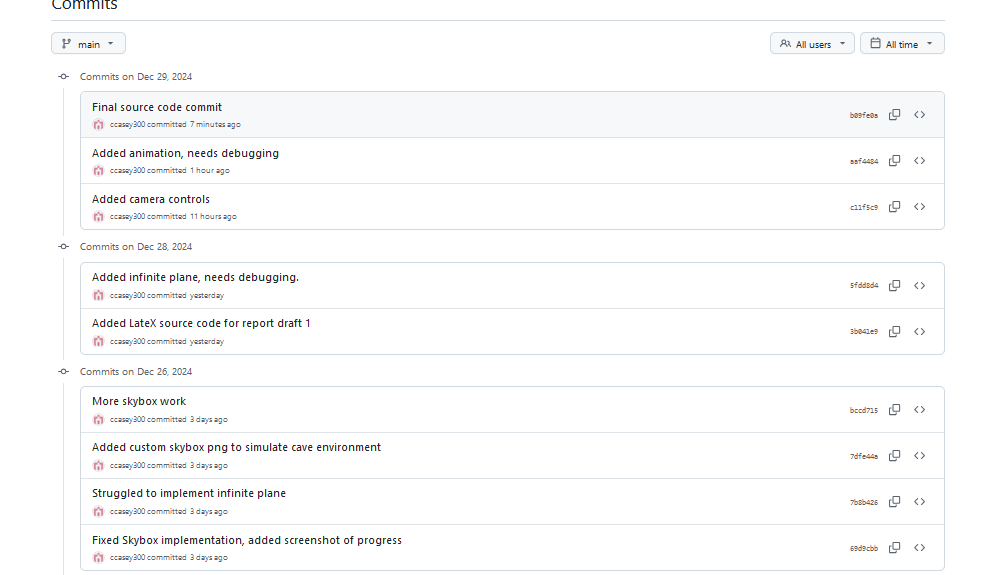
\includegraphics[width=0.5\linewidth]{Results//Progress_screenshots/Git History 2 (top of page)}
    \caption{This screenshot shows the  Git repository history (1/2).}
    %\label{fig:enter-label}
\end{figure}

\begin{figure}
    \centering
    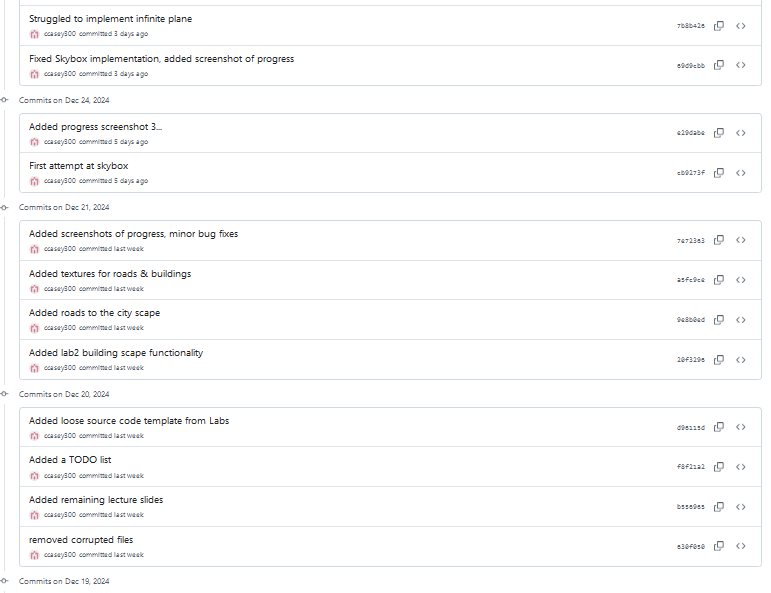
\includegraphics[width=0.5\linewidth]{Results//Progress_screenshots/Git History 1}
    \caption{This screenshot shows the  Git repository history (2/2).}
    %\label{fig:enter-label}
\end{figure}

\newpage
\section*{\Huge{Progress: Description of Screenshots}}

Screenshot 1: Geometry Rendering

Screenshot 2: Texturing and SkyBox

Screenshot 3: Custom SkyBox

Screenshot 4: Lighting and Shadows attempt

Screenshot 5: Animation attempt

Screenshot 6: Final Render


\newpage

\begin{figure}
    \centering
    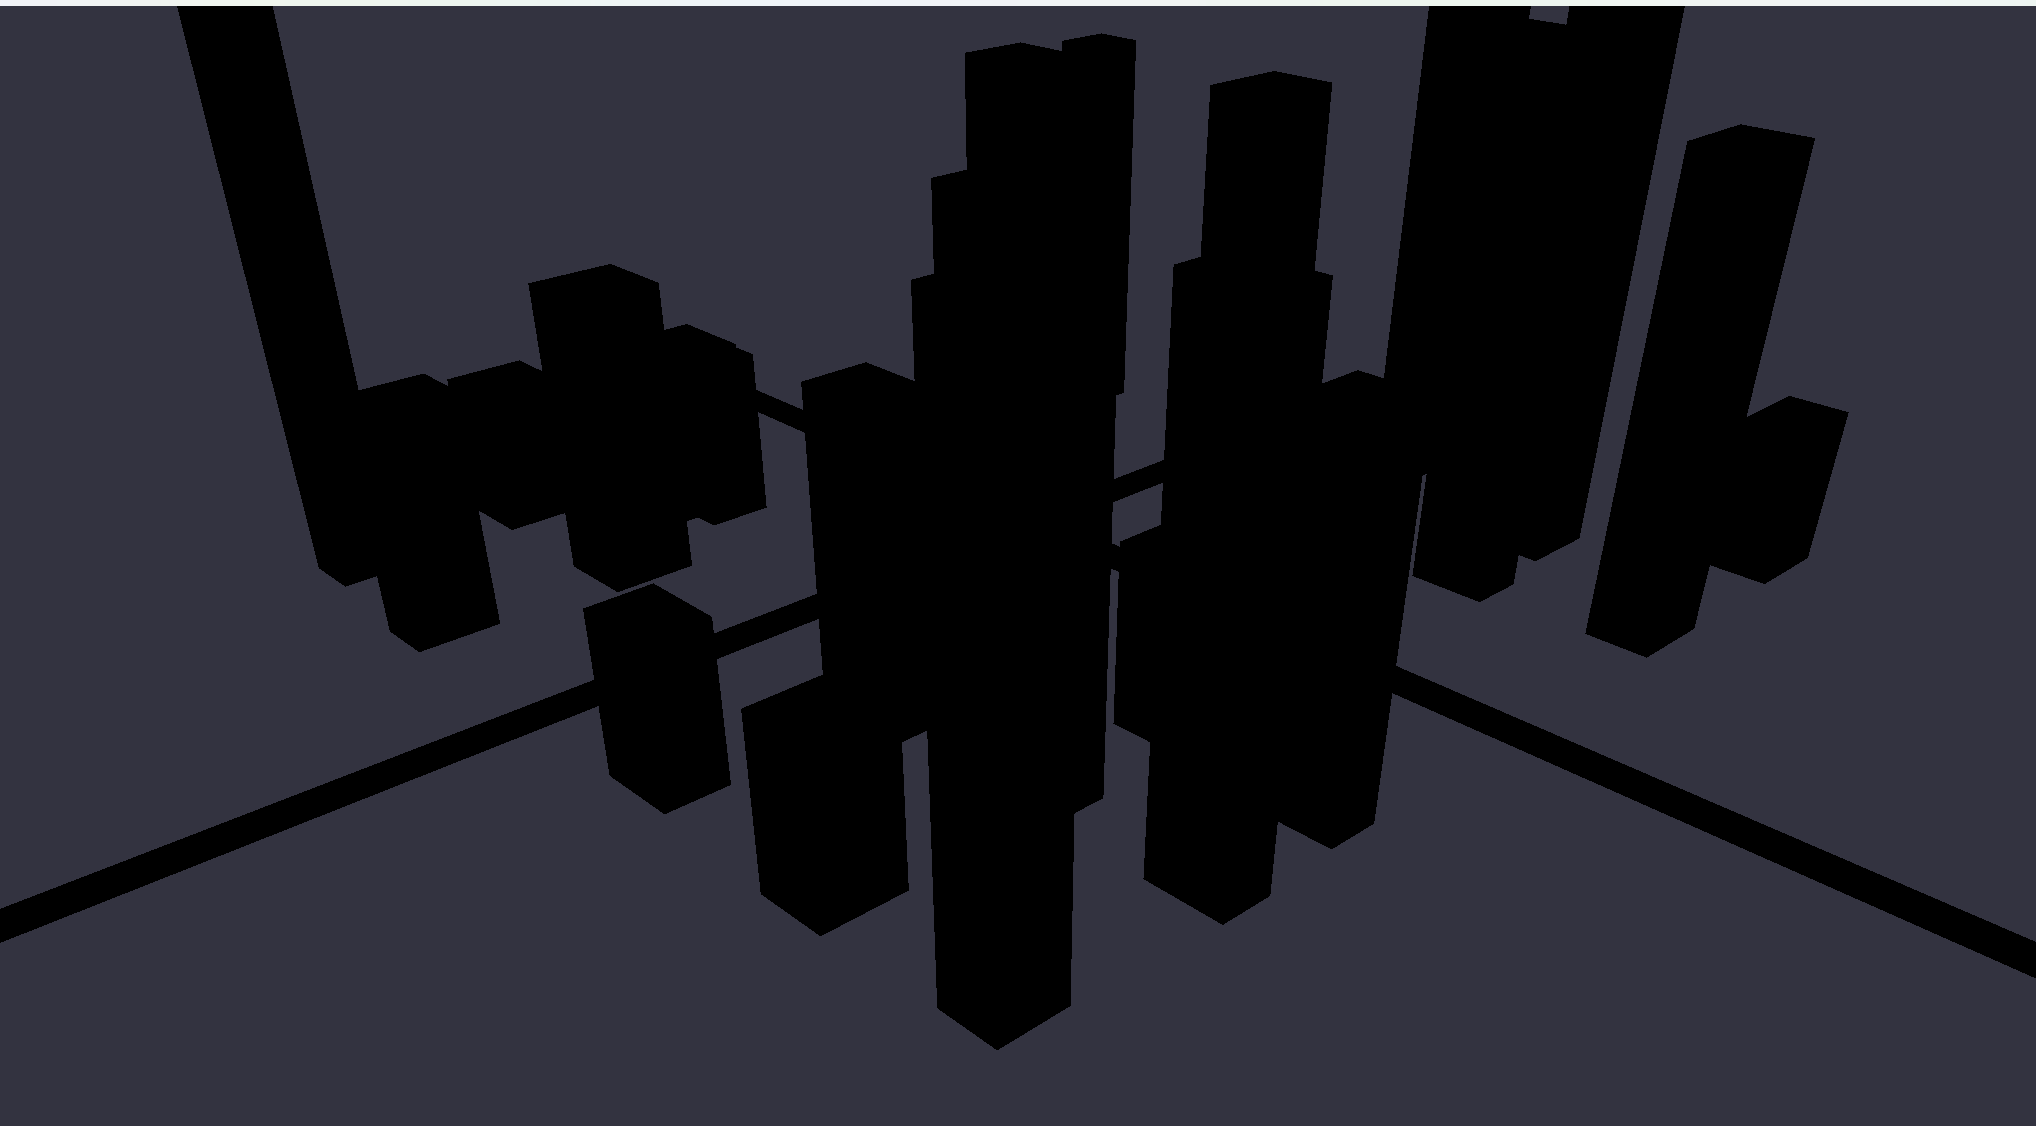
\includegraphics[width=0.5\linewidth]{Results//Progress_screenshots/Screenshot 1 - Geometry.png}
    \caption{This screenshot shows successful rendering of buildings and roads in the scene.}
    %\label{fig:enter-label}
\end{figure}
\begin{figure}
    \centering
    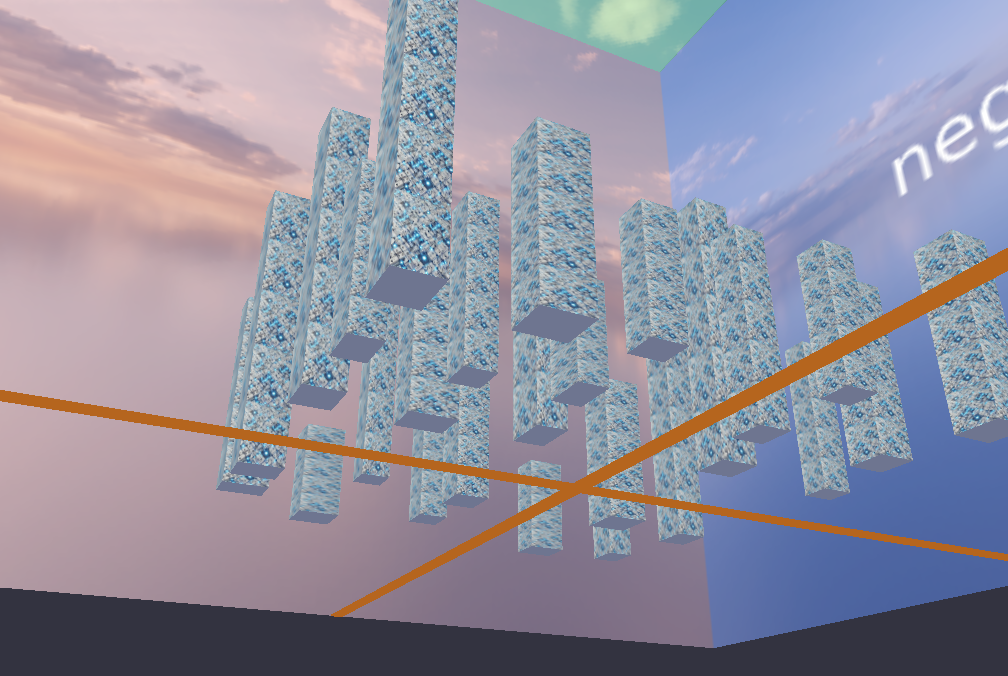
\includegraphics[width=0.5\linewidth]{Results//Progress_screenshots/Screenshot 3a - Skybox.png}
    \caption{This screenshot shows texturing of objects (buildings and roads), and implementation of skybox debug from lab 2.}
    %\label{fig:enter-label}
\end{figure}
\begin{figure}
    \centering
    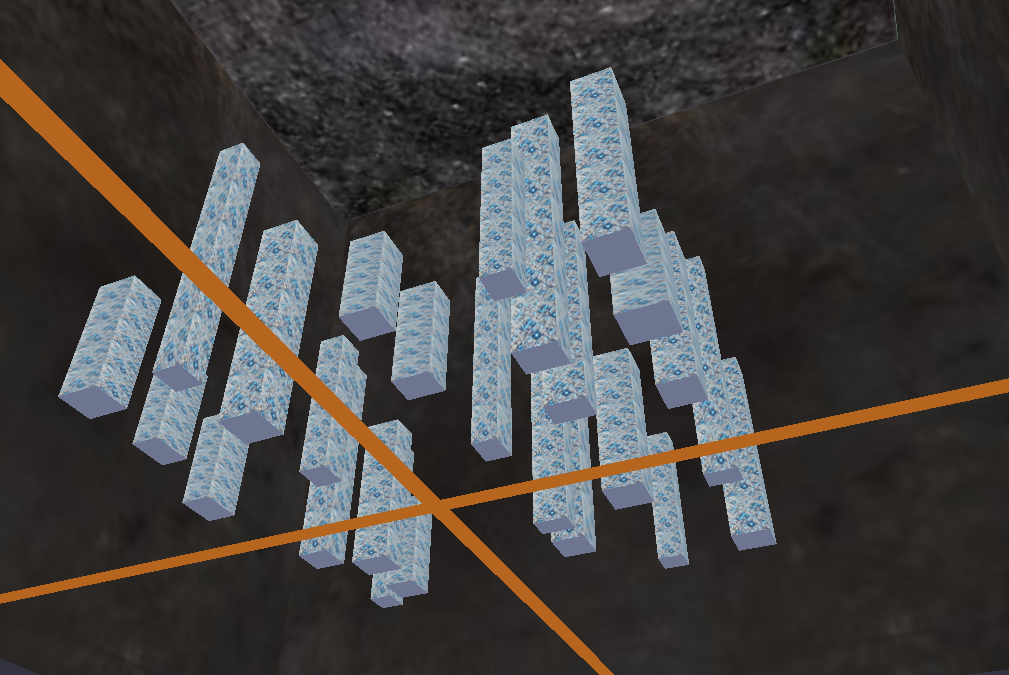
\includegraphics[width=0.5\linewidth]{Results//Progress_screenshots/Screenshot 3b - Custom Skybox.png.png}
    \caption{This screenshot shows a custom "cave themed" SkyBox. This was created using online resources like Adobe Image Editor and free-use google images.}
    %\label{fig:enter-label}
\end{figure}
\begin{figure}
    \centering
    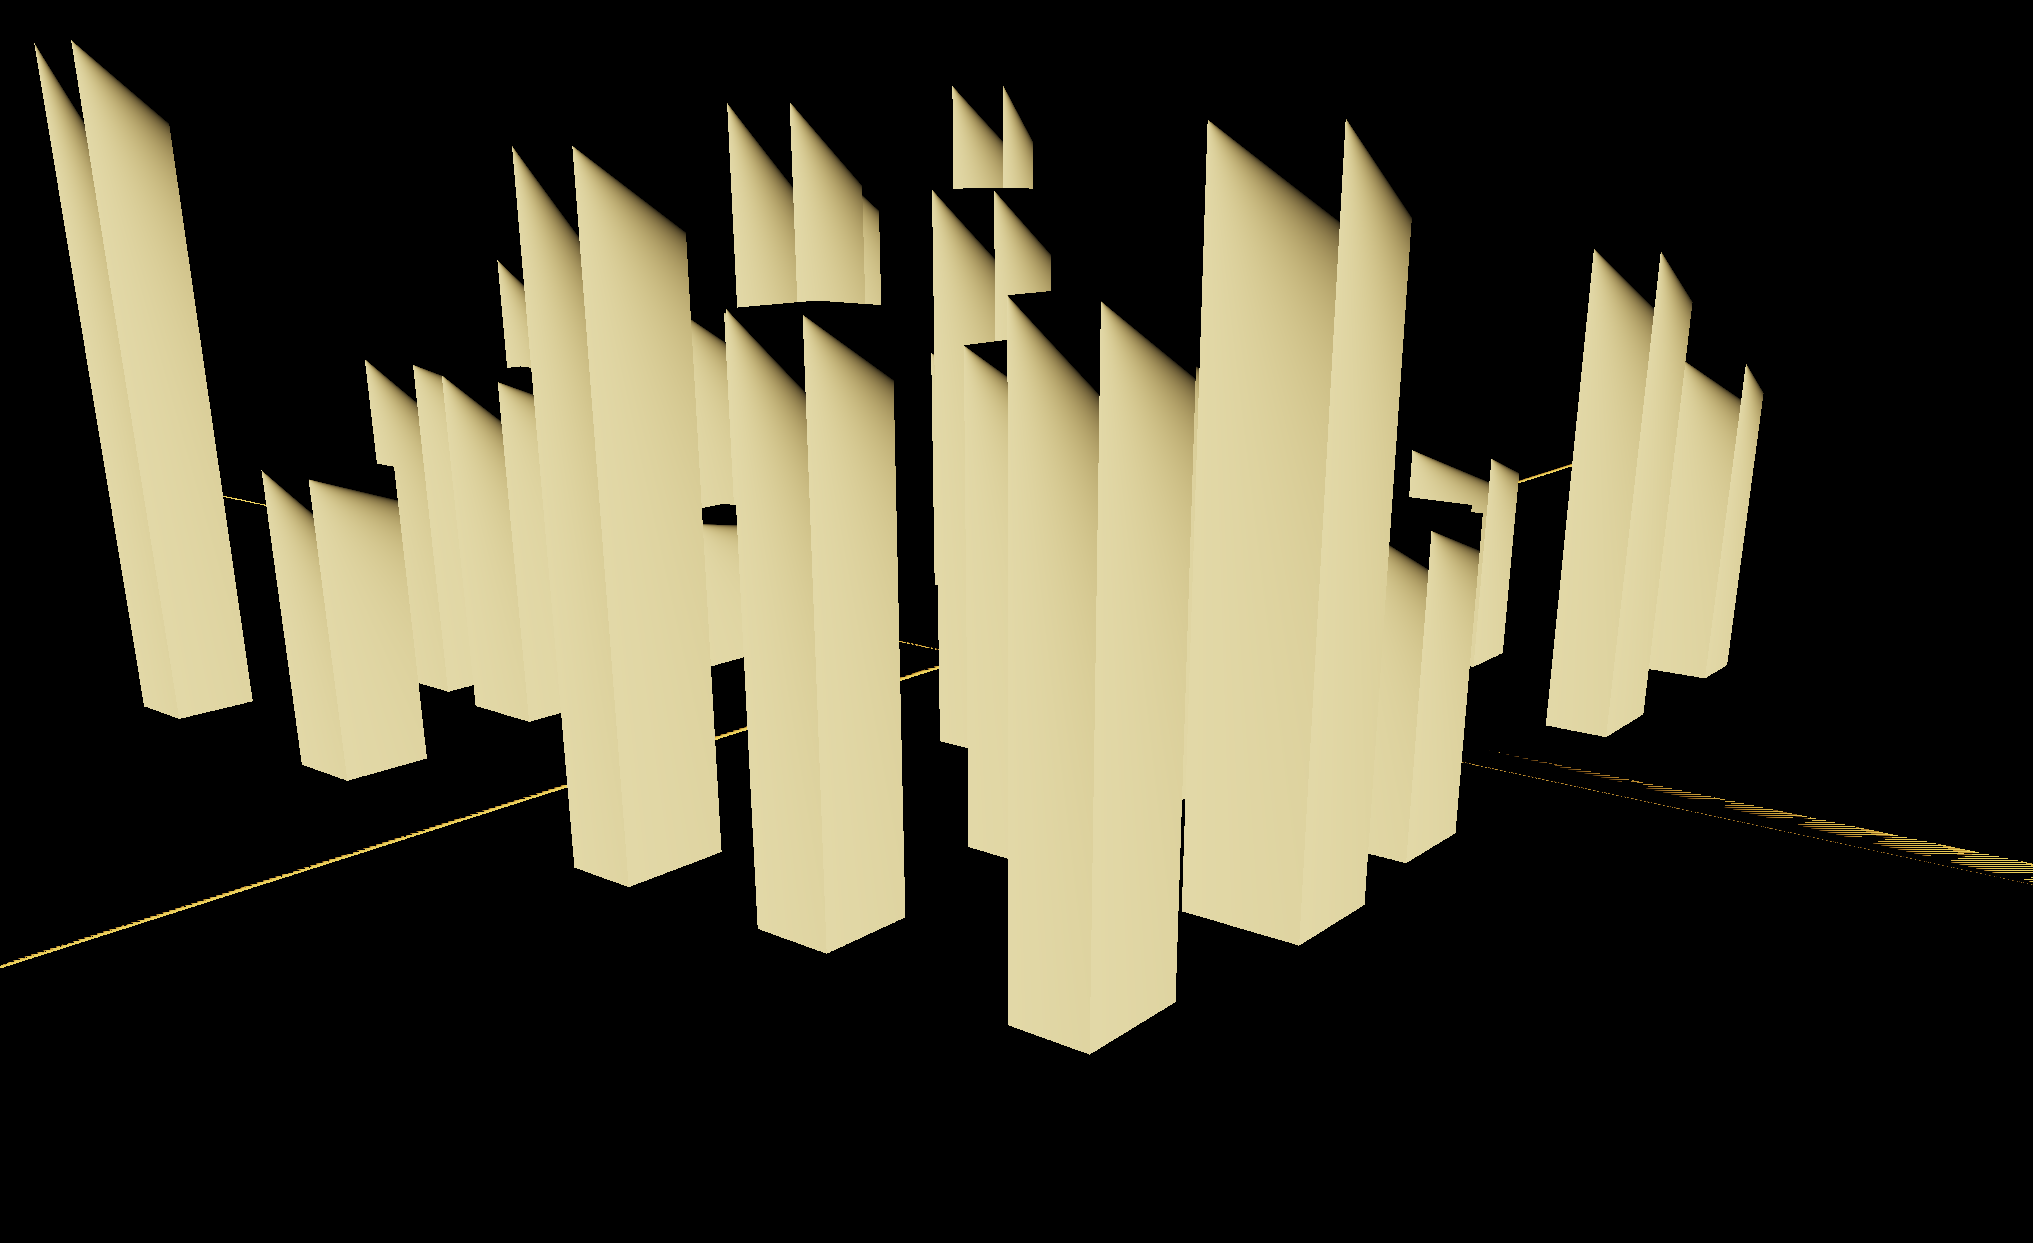
\includegraphics[width=0.5\linewidth]{Results//Progress_screenshots/Screenshot 4 - Lighting & Shadows Attempt.png}
    \caption{My attempt at lighting and shadows, progress can be seen but ultimately could not integrate with textures.}
    \label{fig:enter-label}
\end{figure}
\begin{figure}
    \centering
    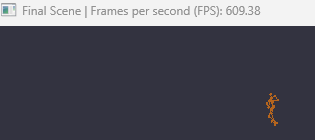
\includegraphics[width=0.5\linewidth]{Results//Progress_screenshots/Screenshot 5 - Animation}
    \caption{My attempt at including animation, could not resolve OGL parameter logic in time}
    \label{fig:enter-label}
\end{figure}
\begin{figure}
    \centering
    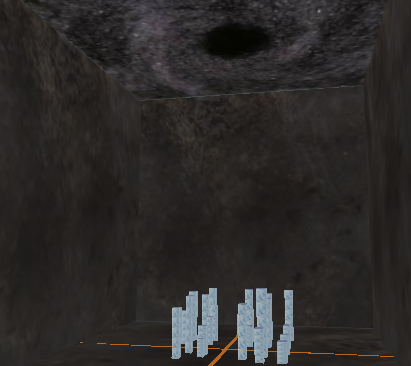
\includegraphics[width=0.5\linewidth]{Results//Progress_screenshots/Screenshot 6 - Final Render}
    \caption{Final render of scene}
    \label{fig:enter-label}
\end{figure}


\newpage
\chapter{Discussion: Quality + Robustness}
I primarily worked using a combination of different lab templates. I primarily used lab 2 and lab 4. However, this approach came with its limitations. Primarily, a lack of object-oriented code as well as being more application specific than I wanted. This lead to lengthy attempts and difficulty debugging. 

As a result, though the code is (maybe) easily understood upon visual inspection, additional elements required a significant amount of work in order to integrate with the existing scene. In this way, I was too dependent on the templates given and should have deviated my approach earlier.

There is some redundant code, several similar structs were defined in order to resolve some texturing issues I faced. If I had more time in the future I would take the existing functionality and try to leverage OOP.



The code includes error-handling much in the same way we did in class. File loading, shader implementation and null pointers are managed appropriately. All cleanup is done after rendering as required. Performance was consistently good, however was never properly challenged. The option to include more animation, more lighting, etc. is there. The scene consistently runs well over 15 FPS on my laptop.
\chapter{Conclusions and Future Work}
%\chapter{Figures, Tables, Referencing}
It is very important to properly refer in the text to any figures, tables or previously published work that you are discussing. Adequate and consistent referencing is one of the criteria which will be used to assess your project report.

\section{Figures}
Graphs, pictures and other images should be included in your report as a numbered, captioned figure. An example is given in Figure \ref{veldis}.

%%%%%%%%%%%%%%%%%%%%%%%%%%%%%%%%%%%%%%%%
\begin{figure}[h]
      \centering
      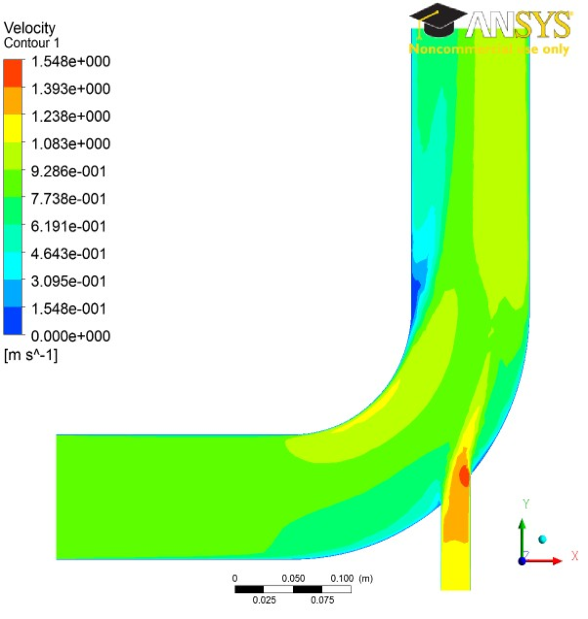
\includegraphics{background/5e1-1.pdf}
      \caption{Velocity distribution on the mid-plane for an inlet velocity for case 1.}
      \label{veldis}
\end{figure}
%%%%%%%%%%%%%%%%%%%%%%%%%%%%%%%%%%%%%%%%

The figure and caption should be centred. The figure numbering starts at 1 at the beginning of each chapter. The caption should provide a brief description of what is being shown. The figure should appear in the document after it is referred to in the text. No figure should be included which is not referred to in the text. Ensure that the size and resolution of images imported from software are sufficient to read any text.

\section{Tables}
Tables are an important way of displaying your results. Table \ref{tab:treatments} is a sample table, adapted from the Master/Doctoral Thesis template at \url{http://www.latextemplates.com/cat/theses}, which was generated with this code:

{\footnotesize
\begin{verbatim}
\begin{table}[b]
\caption{The effects of treatments X and Y on the four groups studied.}
\label{tab:treatments}
\centering
\begin{tabular}{l l l}
\toprule
\textbf{Groups} & \textbf{Treatment X} & \textbf{Treatment Y} \\\midrule
1 & 0.2 & 0.8\\
2 & 0.17 & 0.7\\
3 & 0.24 & 0.75\\
4 & 0.68 & 0.3\\
\bottomrule\\
\end{tabular}
\end{table}
\end{verbatim}
}

\begin{table}[b]
\caption{The effects of treatments X and Y on the four groups studied.}
\label{tab:treatments}
\centering
\begin{tabular}{l l l}
\toprule
\textbf{Groups} & \textbf{Treatment X} & \textbf{Treatment Y} \\
\midrule
1 & 0.2 & 0.8\\
2 & 0.17 & 0.7\\
3 & 0.24 & 0.75\\
4 & 0.68 & 0.3\\
\bottomrule\\
\end{tabular}
\end{table}

Tables are numbered in the same way as figures. Typically tables also have a short caption, but this is not universally true. The number and caption appear above the table, not below as with figures. Again, no table should appear in the report which has not been referred to in the text. Tables should come after they are discussed in the text. The exact formatting of the table depends somewhat on the content of the table, but in general, the text in the table should be the same font and size as the main text. 

\section{Equations}
All equations should be numbered sequentially. Do not restart the numbering at the beginning of each chapter. Unlike figures and tables, you may not need to refer to every equation in the text. You should take care to format equations properly. Do no simply try to use plain text. Use the equation layout facilities. An example of how equations should appear is shown in Equation \ref{sampleequation}. Here is the code for it:

{\footnotesize
\begin{verbatim}
\begin{equation}
\textrm{div}(\underline{u}) = \frac{\delta u}{\delta x} + \frac{\delta v}{\delta y} +
        \frac{\delta w}{\delta z} = 0
\label{sampleequation}
\end{equation} 
\end{verbatim}
}

\begin{equation}
\textrm{div}(\underline{u}) = \frac{\delta u}{\delta x} + \frac{\delta v}{\delta y} + \frac{\delta w}{\delta z} = 0
\label{sampleequation}
\end{equation} 

\section{Referencing published work}
It is important to give appropriate credit to other people for the work that they have shared through publications. In fact, you must sign a declaration in your report stating that you understand the nature of plagiarism. As well as avoiding plagiarism, citing results or data from the literature can strengthen your argument, provide a favourable comparison for your results, or even demonstrate how superior your work is.

There are many styles to reference published work. For example, the parenthetical style (which is also called the \emph{Harvard style}) uses the author and date of publication (e.g. ``Smith and Jones, 2001''). There is also the Vancouver style (or the \emph{citation sequence style}), which is used in this document. In the Vancouver style, the publications are cited using bracketed numbers which refer to the list in the References section at the end of the report. The references are listed in the order that they are cited in the report. A variant is \emph{name sequence style}, in which the publications are referenced by number, but the list is arranged alphabetically. The following paragraph shows the use of the Vancouver style: 

\begin{quote}
Several studies have examined the sound field around tandem cylinders generated by flow\cite{fitzpatrick2003flow,finnegan2010experimental}, while other investigations have focused on the effect of an applied sound field on the flow\cite{hall2003vortex}. Papers from conference proceedings\cite{jordan2001array}, books\cite{paidoussis2010fluid} and technical reports\cite{reyes2007power} can be dealt with in the same style.
\end{quote}

The Vancouver style has the advantage that it is a little more compact in the text and does not distract from the flow of the sentence if there are a lot of citations. However, it has the disadvantage that it is not immediately clear to the reader what particular work has been referenced.

It actually does not matter which particular referencing style is used as long as three important considerations are observed:
\begin{itemize}
\item the referencing style used throughout the document is consistent;
\item all material used or discussed in the text is properly cited;
\item nothing is included in the reference list that has not been cited.
\end{itemize}

This template has a suitable referencing style already set up -- you should use it and use the built-in BibTeX system to manage your references. See above for examples of how to cite a reference and look in the \texttt{sample.bib} file to see BibTeX references. Remember \href{http://scholar.google.com}{Google Scholar} and other search engines will give you BibTeX references for lots of academic publications. Otherwise, you can easily make up your own based on the examples in that file.
%\chapter{\LaTeX}
\label{latexchapter}
\LaTeX{}, or more properly ``\LaTeXe{}'', is a very useful document processing program. It is very widely used, widely available, stable and free. Famously, \TeX, upon which \LaTeX{} is built, was originally developed by the eminent American mathematician Donald Knuth because he was tired of ugly mathematics books \cite{shustek2008interview}. Although it has a learning curve (made much less forbidding by online tools and resources -- see below), it allows the writer to concentrate more fully on the content, and takes care of most everything else.

While it can be used as a word processor, it is a \emph{typesetting} system, and Knuth's idea was that it could be used to produce beautiful looking books:
\begin{quote}
\emph{\LaTeX{} is a macro package which enables authors to typeset and print their work at the highest typographical quality, using a predefined, professional layout.}\footnote{This is from \citet{oetiker2001not}. Did we mention that you should minimise your use of footnotes?}
\end{quote}
\LaTeX{} has great facilities for setting out equations and a powerful and very widely supported bibliographic system called BibTeX, which takes the pain out of referencing.

Three useful online resources make \LaTeX~much better:
\begin{enumerate}[(1)]
\item An excellent online \LaTeX{} environment called ``Overleaf'' is available at \url{http://www.overleaf.com} and runs in a modern web browser. It's got this template available -- search for a TCD template. Overleaf can work in conjunction with Dropbox, Google Drive and, in beta, GitHub.
\item Google Scholar, at \url{http://scholar.google.com}, provides BibTeX entries for most of the academic references it finds.
\item An indispensable and very fine introduction to using \LaTeX{} called \emph{``The not so short introduction to LATEX 2$\varepsilon$''} by \citet{oetiker2001not} is online at \url{https://doi.org/10.3929/ethz-a-004398225}. Browse it before you use \LaTeX~for the first time and  read it carefully when you get down to business.
\end{enumerate}
Other tools worth mentioning include:
\begin{itemize}
\item \texttt{Draw.io} -- an online drawing package that can output PDFs to Google Drive -- see \url{https://www.draw.io}.
\end{itemize}
%\bibliographystyle{unsrtnat}
%\bibliography{bibs/sample}
%\appendix
\newpage
\section*{\Huge{Acknowledgements}}


AI models used for debugging and creating interesting objects:

GPT 3.0

GitHub CoPilot (GPT 3.0 also I believe)

Resources used:

OpenGL Tutorials http://www.opengl-tutorial.org/

Infinite plane attempt https://www.youtube.com/@OGLDEV

Lecture notes, labs, etc. Binh-Son Hua 

\newpage \tableofcontents
\renewcommand{\thechapter}{A\arabic{chapter}}
%\chapter{Appendix}
You may use appendices to include relevant background information, such as calibration certificates, derivations of key equations or presentation of a particular data reduction method. You should not use the appendices to dump large amounts of additional results or data which are not properly discussed. If these results are really relevant, then they should appear in the main body of the report.

\section{Appendix numbering}
Appendices are numbered sequentially, A1, A2, A3\ldots The sections, figures and tables within appendices are numbered in the same way as in the main text. For example, the first figure in Appendix A1 would be Figure A1.1. Equations continue the numbering from the main text.



\end{document}